\documentclass{ximera}

%\addPrintStyle{..}

\begin{document}
	\author{Bart Lambregs}
	\xmtitle{Oplossingsstrategie}{}
    \xmsource\xmuitleg





	%%%\section{Oplossingsstrategie}

	Bij het oplossen van vraagstukken waarin de wetten van Newton worden gebruikt, kan een vast stramien of heuristiek gebruikt worden. Omdat elke opgave anders is, blijft creativiteit noodzakelijk.
	\begin{enumerate}
	\item Bepaal het systeem dat je wilt beschouwen. Kies een systeem (object, lichaam, massa, geheel van lichamen) waarvan je een onbekende kracht of versnelling wilt berekenen. Kies een samengesteld systeem als je hierover informatie hebt.
	\item Maak het systeem vrij. Beschouw het systeem als een vrij lichaam waarop alle uitwendige krachten inwerken. Teken al deze krachten die op het systeem werken. Dus niet de krachten die het systeem op zijn omgeving uitoefent. Die grijpen immers aan op een ander object. Het systeem waarop alle uitwendige krachten zijn getekend, wordt ook wel een krachtendiagram genoemd.
	\item Pas de tweede wet van Newton toe op het systeem. Dit betekent dat de som van alle uitwendige krachten gelijk is aan de massa van het beschouwde systeem vermenigvuldigd met zijn versnelling:
	\begin{eqnarray*}
	\sum_{i=1}^n\vec{F}_i=m\vec{a}
	\end{eqnarray*}
	\item Kies een referentiestelsel en projecteer de vectorvergelijking. Ontbind de vectorvergelijking a.h.v. de eenheidsvectoren volgens de assen van een goed gekozen referentiestelsel. Op die manier bekom je
	twee vergelijkingen die equivalent zijn met de vectorvergelijking:
	\begin{eqnarray*}
	x-as&:&\sum_{i=1}^nF_{i,x}=ma_x\\
	y-as&:&\sum_{i=1}^nF_{i,y}=ma_y
	\end{eqnarray*}
	Hierin zijn $F_{i,x}$ en $F_{i,y}$ de componenten van de verschillende krachten volgens respectievelijk de $x$-as en de $y$-as.
	\item Kies een tweede, derde \ldots systeem en herhaal stap 1 t/m 4. Indien er meer dan \'e\'en onbekende is, moet je nog andere systemen beschouwen. Kies ze zodanig dat je de derde wet van Newton kunt gebruiken tussen de verschillende systemen of dat de versnelling dezelfde is.
	\item Los het stelsel vergelijkingen op.
	\end{enumerate}
	
	%%\newpage
	
	% \voorbeeld{}{\textsf{
	\begin{exercise}
	Twee massa's $m_1$ en $m_2$ zijn via een touwtje en een katrol van te verwaarlozen massa met elkaar verbonden zoals in de figuur. Er is geen wrijving aanwezig. De massa's hebben een versnelling zoals aangegeven.
	%%%\newline
	Bepaal de grootte van de versnelling van beide massa's en de grootte van de spankracht in het touw.
	\begin{image}
	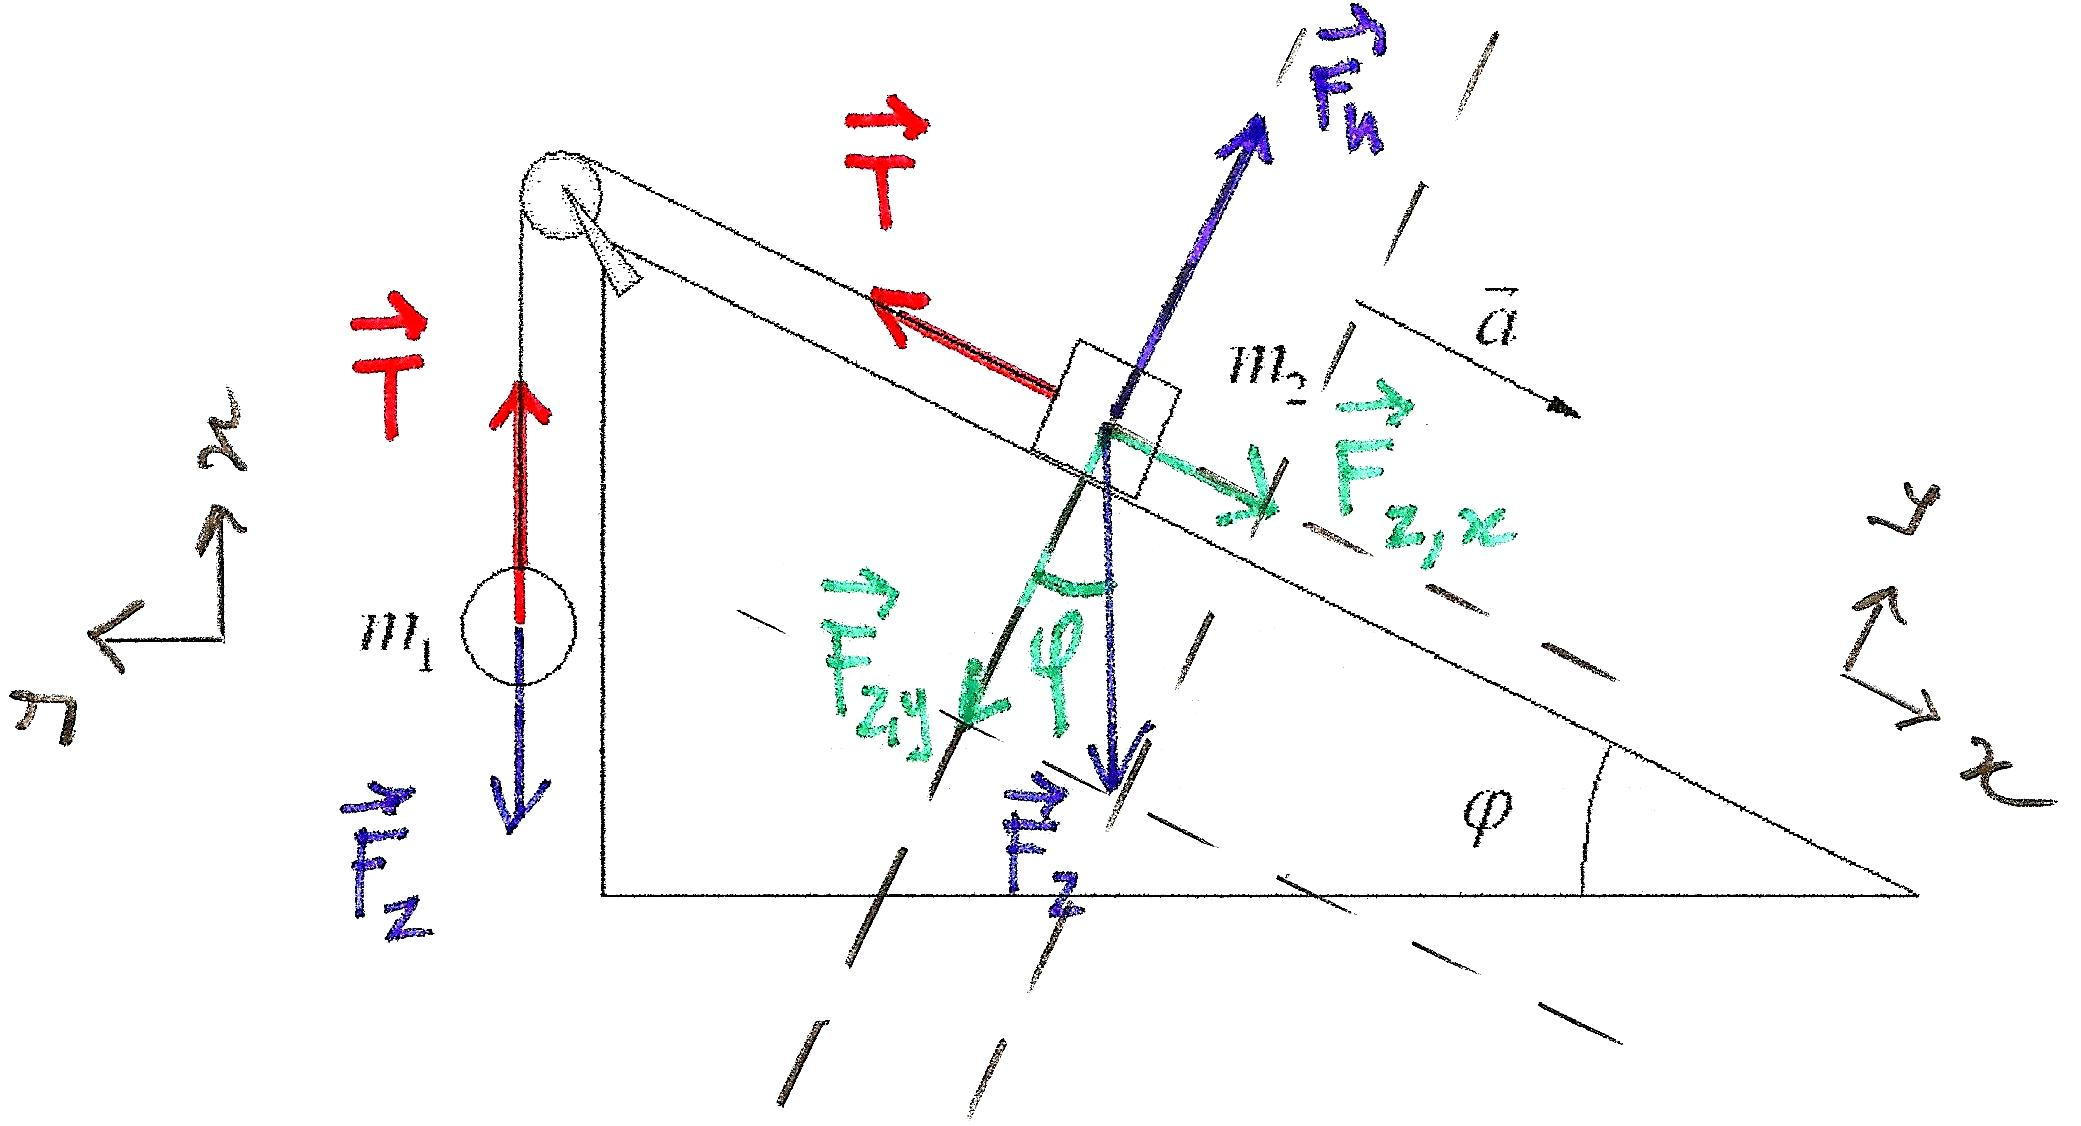
\includegraphics[width=0.45\textwidth, angle=0]{blokken_helling_opl}
	\end{image}

	\begin{oplossing}
	% \item[gegeven]$m_1,~m_2,~\varphi$
	% \item [gevraagd]$a$, $F_s$
	% \item [oplossing]
	De tweede wet van Newton toepassen op $m_1$ levert
	\begin{eqnarray}
	F_s-m_1g&=&m_1a\nonumber\\
	&\Updownarrow&\nonumber\\
	F_s&=&m_1(a+g)
	\end{eqnarray}
	De tweede wet van Newton toepassen op $m_2$, met $F_z=mg$, levert
	\begin{eqnarray}
	F_{z,x}-F_s&=&m_2a\nonumber\\
	&\Updownarrow&\nonumber\\
	F_s&=&m_2(g\sin{\varphi}-a)
	\end{eqnarray}
	Uit (\ref{T1}) en (\ref{T2}) volgt
	\begin{eqnarray}
	%m_1(a+g)&=&m_2(g\sin{\varphi}-a)\nonumber\\
	%&\Updownarrow&\nonumber\\
	a&=&\frac{m_2\sin{\varphi}-m_1}{m_1+m_2}g\nonumber
	\end{eqnarray}
	Dit resultaat substitueren in (\ref{T2}) levert, na het uitwerken door op ge\-lij\-ke noemer te zetten:
	\begin{eqnarray}
	F_s&=&\frac{m_1m_2g(1+\sin{\varphi})}{m_1+m_2}\nonumber
	\end{eqnarray}
	\end{oplossing}
	\end{exercise}
	% }}
	
	
	%%\newpage
	

\end{document}
